%&LaTeX

\section{Signals in the Computer}

In this lab, you will use JDSP to explore how a physical signal can
be considered to be composed of a sum of sinusoids --- its
\emph{Fourier series}. You will then investigate how capturing this
signal for computer use --- sampling and quantization --- modifies the
signal. Finally, you will see how the choices you make in the
parameters for sampling and quantization affect the quality of the
digitized, computer signal. 



\subsection{Fourier series representation of a physical signal}
	In this section, you will use the  \block{Cont Sig} block in J-DSP to simulate a analog signal 
	generator. The \block{Cont 
	Sig} block is capable of simulating analog signals of varying frequency content. 
	
	% Block diagram, step 1
	\begin{figure}[b]
	  \begin{center}
	    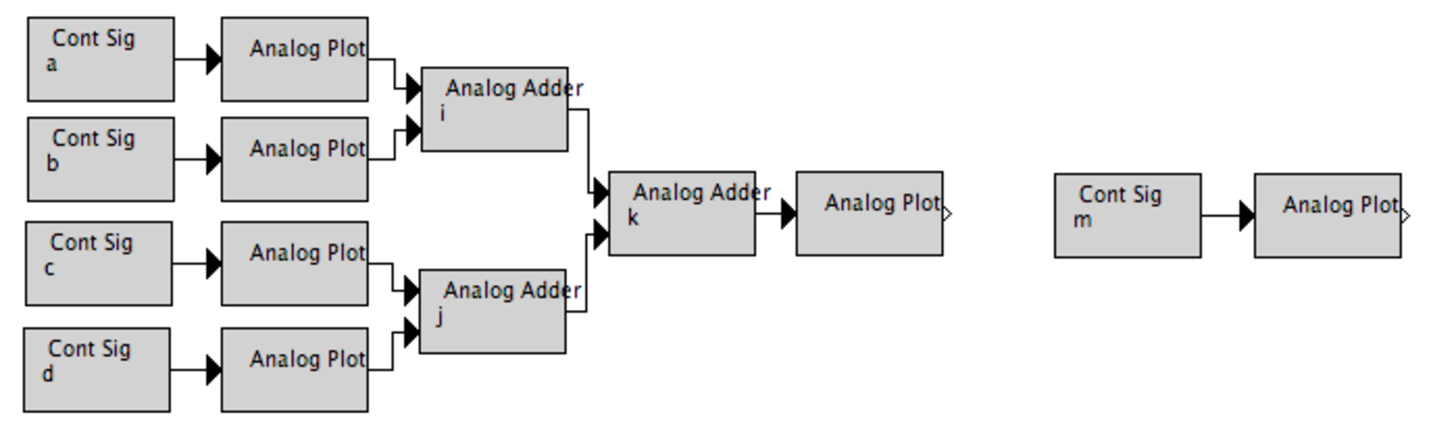
\includegraphics[height=1.5in]{lab3/block_diagram_step1}
	  \end{center}
	\caption{ A J-DSP diagram for summing and plotting analog sine waves (left) and a single 
	triangle wave (right). 
	\label{fg:step1}}
	\end{figure}

\paragraph{Step 1.1} Create a J-DSP diagram that sums together four continuous time sinusoids 
	and plots their sum. Use the ``Analog Blocks'' function set and the \block{Adder} block only (See 
	Figure \ref{fg:step1}). Also create a separate set of blocks that plots a continuous time triangle 
	wave at a \option{frequency} of 200 Hz and \option{amplitude} of 1. In the next section you will 
	simulate this triangle wave using the sum of sinusoids.

\paragraph{Step 1.2} Recall that any periodic signal can be represented as a sum of harmonic 
	sinusoids. The amplitude of each harmonic is known as the Fourier Series. It may at first seem
	like sums of sinusoids would be poor approximations of real periodic signals, but this is not 
	the case. We
 	can illustrate this using a triangle wave. The formula for synthesis of a triangle wave with 
	frequency $\omega_0$ is a sum of harmonically related sine waves (its Fourier series):
	\[
	x(t) = \sum_{k=0}^{\infty}
	\left( 
	\underbrace{ \frac{8}{\pi^2} \frac{(-1)^k}{(2k+ 1)^2} }_{ \text{amplitude} } 
	\underbrace{ \sin((2k+1)\omega_0 t) }_{ (2k+1)^{th}\text{ harmonic} } 
	\right)
	\]
	In this case, in the analog domain, we are dealing with frequencies in
	Hz, and so $\omega_0 = 2\pi f_0$. Notice that the Fourier Series of the triangle wave only uses 
	odd harmonics (i.e., the only non-zero frequencies are $(2k+1)\omega_0=\omega_0, 3\omega_0, 
	5\omega_0 \cdots$). Also notice that resulting wave will be zero mean because there is no ``DC'' 
	term (i.e., $2k+1 \neq 0$ for any integer k). 
	Use your diagram from Step 1.1 to generate and sum the
	first 7 harmonics of the Fourier Series of a triangle wave and plot the resultant signal (i.e., use 
	$f_0$, $2f_0$, $3f_0$, $\cdots 7f_0$, where $f_0=$200 Hz). How does this signal compare to 
	the triangle wave computed directly in \block{Cont. Sig}?
	

\paragraph{Step 1.3} Another way to view a signal is in the \emph{frequency domain}. For a 
	signal expressed in terms of its Fourier Series, the \emph{frequency domain} representation
	is merely the coefficients of the harmonics. Use your favorite spreadsheet or plotting tool to 
	compute and plot 
	the spectrum of a triangle wave.  Note that you are \emph{not} being asked to plot the triangle 
	wave as a function of time; you should plot the amplitudes of the Fourier Series as a 
	function of the harmonics' frequencies (like the vertical lines in textbook figure~1.12).  
	


\subsection{Sampling}

	The first step in digitization is \emph{sample and hold}, in which the
	continuous analog signal is converted to a \textit{discrete-time} analog signal
	(an analog signal that only changes its value at particular points in
	time). You will use the \block{Sample-Hold} block in J-DSP to simulate this.
	
	% Block diagram, step 2
	\begin{figure}[h]
	  \begin{center}
	    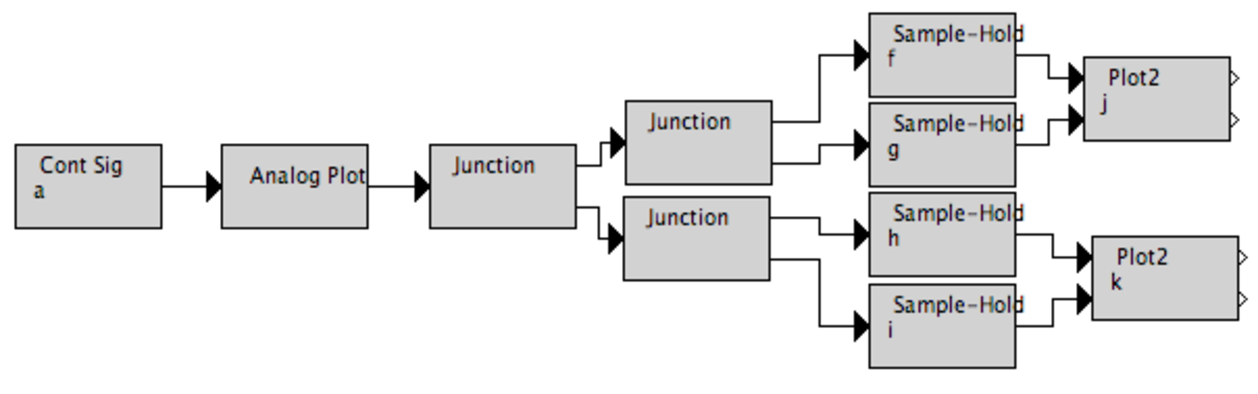
\includegraphics[height=1.5in]{lab3/block_diagram_step2}
	  \end{center}
	\caption{ A J-DSP diagram for investigating sampling rate. \label{fg:step2}}
	\end{figure}

\paragraph{Step 2.1} Create an \block{Cont Sig} sine waveform ranging
	from -5 to 5V with a frequency of 200Hz (Figure \ref{fg:step2}, leftmost block).

\paragraph{Step 2.2} Use four \block{Sample-Hold} blocks to sample
	this signal at 300Hz, 500Hz, 1000Hz and 2000Hz. Plot the original and all four sampled signals 
	separately (Figure \ref{fg:step2}). Does it appear that all sampled versions are equally useful in 
	representing the original? If not, explain why.
	

\subsection{Analog to Digital Conversion}

	The last step of digitization is called ``analog to digital conversion,'' or \emph{quantization}. In 
	this step, the sampled analog signal is converted to a discrete signal, with values represented 
	by $b$ bit integers. We will use the \block{Quantizer} block under the ``Statistical DSP'' function 
	set to perform this conversion.
	
	% Block diagram, step 3
	\begin{figure}[h]
	  \begin{center}
	    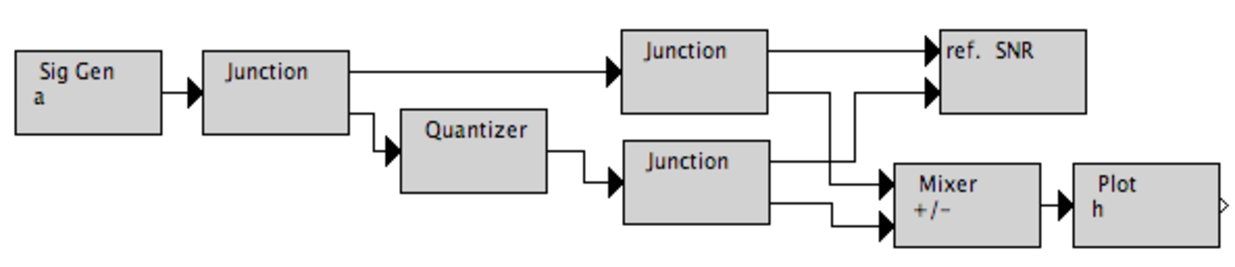
\includegraphics[width=5.0in]{lab3/block_diagram_step3}
	  \end{center}
	\caption{ A J-DSP diagram for investigating quantization error and calculating SNR. 
	\label{fg:step3}}
	\end{figure}

\paragraph{Step 3.1} Next we will be using the \block{SNR} block under the ``Basic Blocks'' 
	function set to compute signal-to-noise ratio (SNR) as a result of quantization. Place the 
	\block{SNR} block and open the dialog associated with it. You will see the equations used to 
	calculate the numerator and denominator. In your own words, what quantity is calculated in the 
	numerator and what quantity is calculated in the denominator of this ratio (Hint: can you 
	describe the values in terms of \emph{root mean square} (RMS) values)? Note that this SNR is 
	different than what we did in the textbook, because we are now doing the computation for a 
	\textit{specific} signal, not just figuring SNR for a possible \textit{range} of signal values.
	

\paragraph{Step 3.2} Use the J-DSP diagram in Figure \ref{fg:step3} to compute the SNR for a 
	quantized sinusoid. Use the \block{SigGen} block with a ``amplitude'' of 5, ``frequency'' of 0.05$
	\pi$, and ``Pulsewidth'' of 256. Use 2, 4, 8, 12, and 16 bits quantization. Use your favorite 
	spreadsheet or plotting software to plot SNR versus number of quantization bits (i.e., a scatter 
	plot). Use the output of \block{SigGen} as reference for the \block{SNR} block. 

\paragraph{Step 3.3} Plot the quantization error by using the \block{Adder} block (bottom right 
	blocks of Figure \ref{fg:step3}). Set the \block{Adder} block to ``subtract'' by opening the dialog 
	and switching the ``$+$'' sign to ``$-$.'' You only need to include the quantization error plot for 
	``4 bits'' in your report (but be sure to view the error plots for all quantization levels).

\paragraph{Step 3.4} Repeat Step 3.2 using a triangle waveform with ``Gain'' of 5 and 
	``Pulsewidth'' of 256. 

\paragraph{Step 3.5} As you double the number of bits used in quantization, how does the SNR 
	change? Refer to specific features of your plots from Steps~3.2--3.4 to justify your answer. 
	

% LocalWords:  WebQ MATLAB
